
\begin{frame}
\frametitle{Detection of Flooded Buildings with Multi-Sensor Data Fusion}
\begin{tikzpicture}[node distance=.1em, inner sep=0, text depth=0pt, label distance=1em]

\node[label={above:0.5m post-disaster}](a){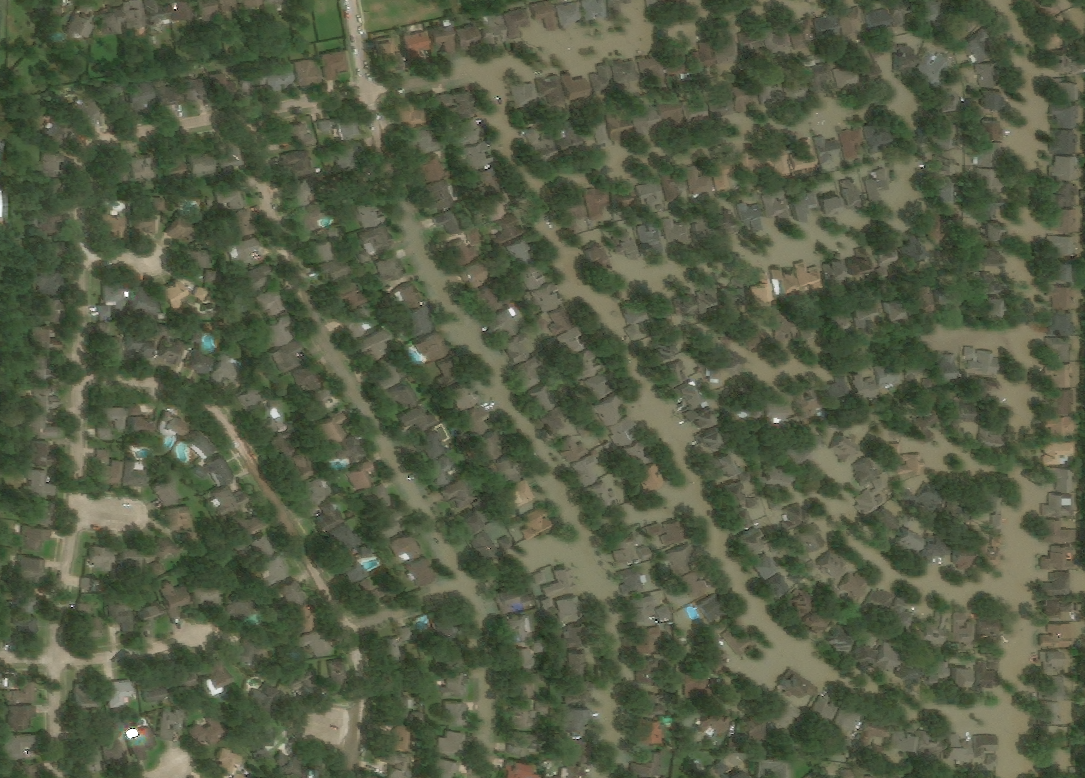
\includegraphics[width=.33\textwidth]{images/resolution_examples/vhr.png}};

\only<1>{\node[right=of a, label=above:10m pre-disaster](b){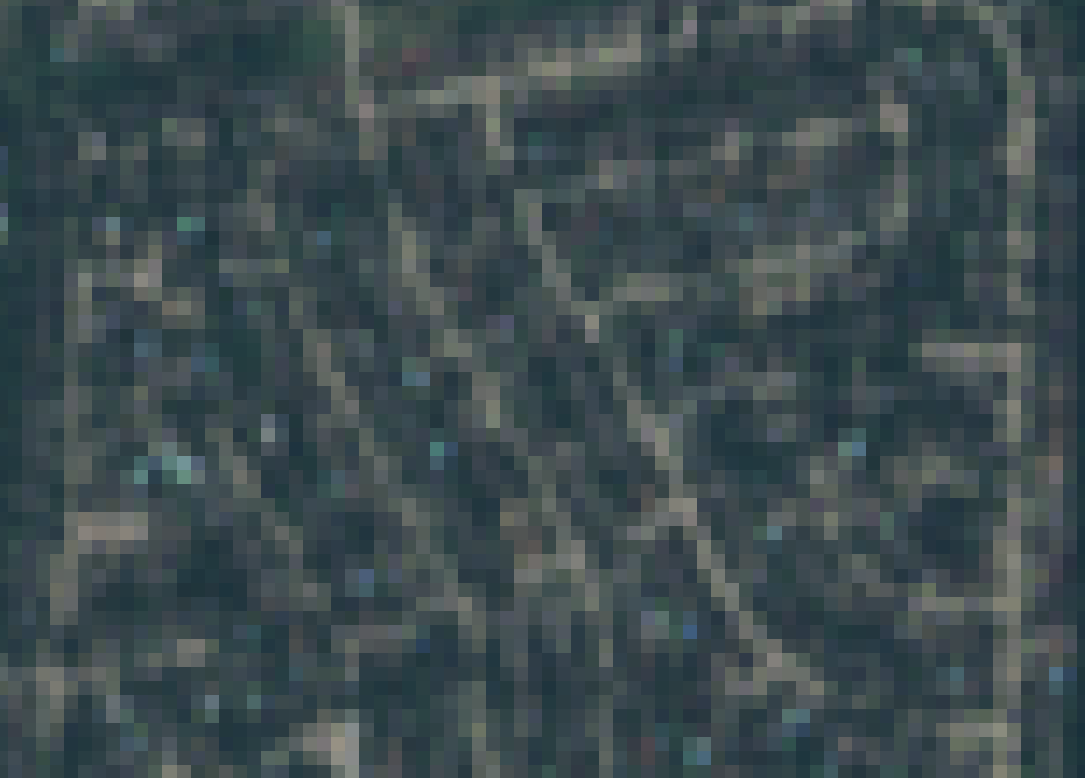
\includegraphics[width=.33\textwidth]{images/resolution_examples/s2_pre.png}};}
\only<2>{\node[right=of a, label=above:10m post-disaster](b){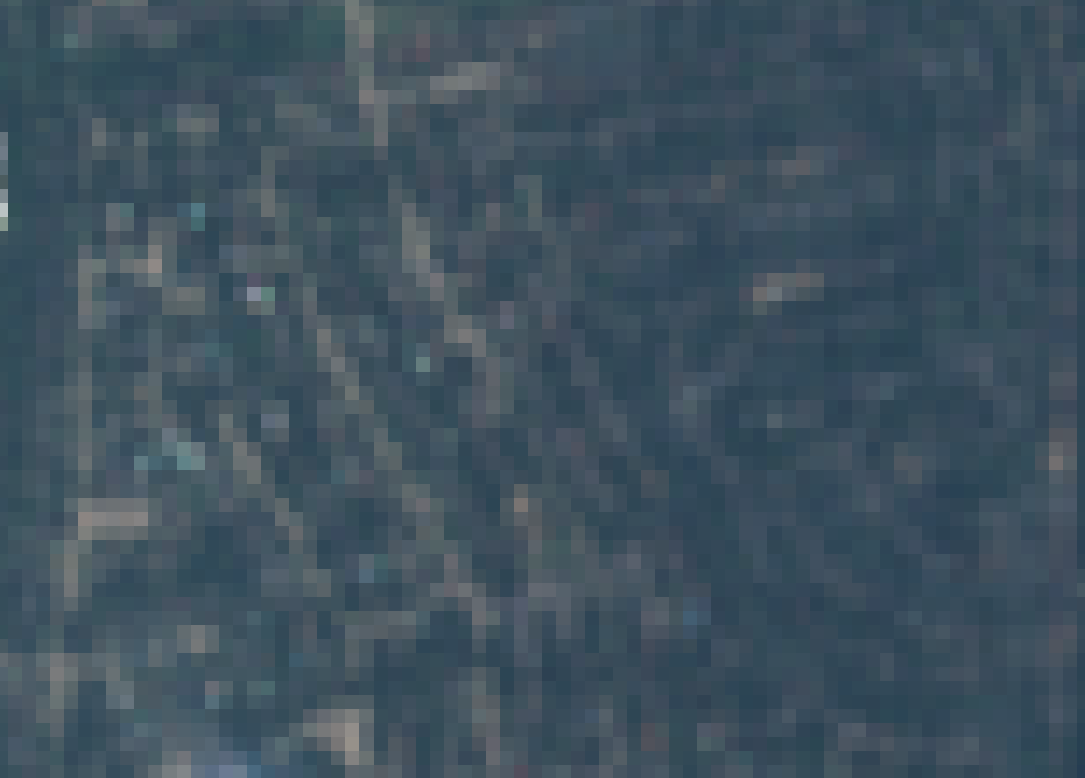
\includegraphics[width=.33\textwidth]{images/resolution_examples/s2_post.png}};}

\only<1>{\node[right=of b, label=above:10m pre-disaster](c){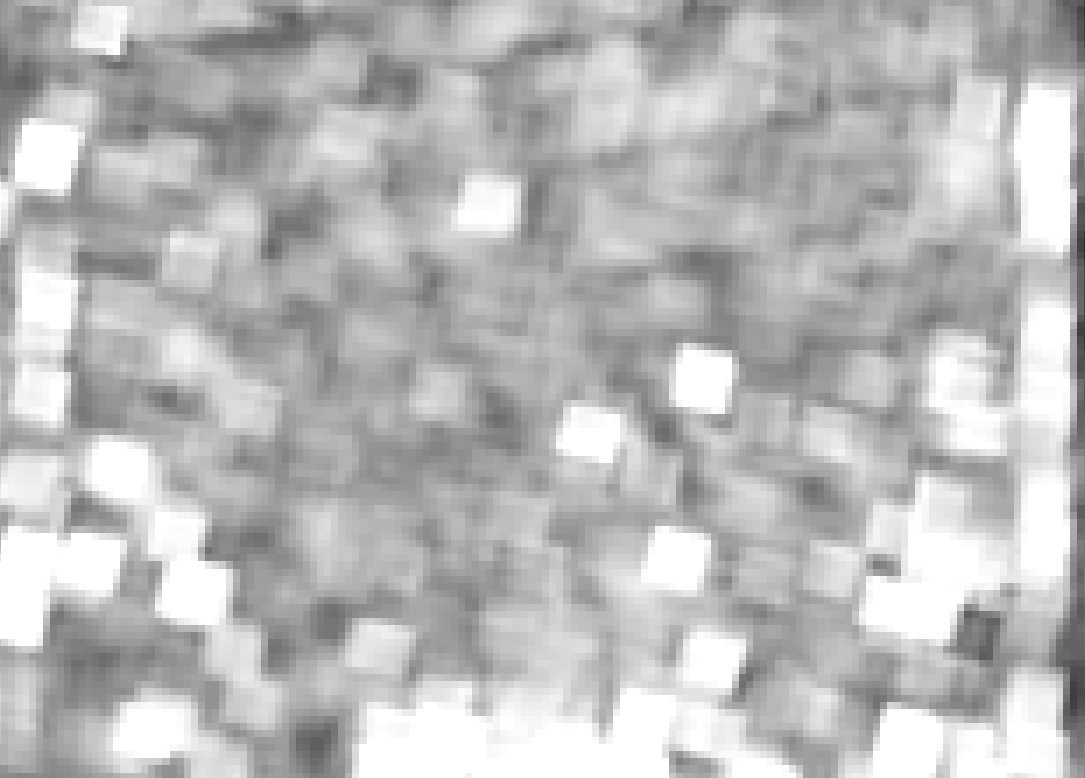
\includegraphics[width=.33\textwidth]{images/resolution_examples/coh_pre.png}};}
\only<2>{\node[right=of b, label=above:10m post-disaster](c){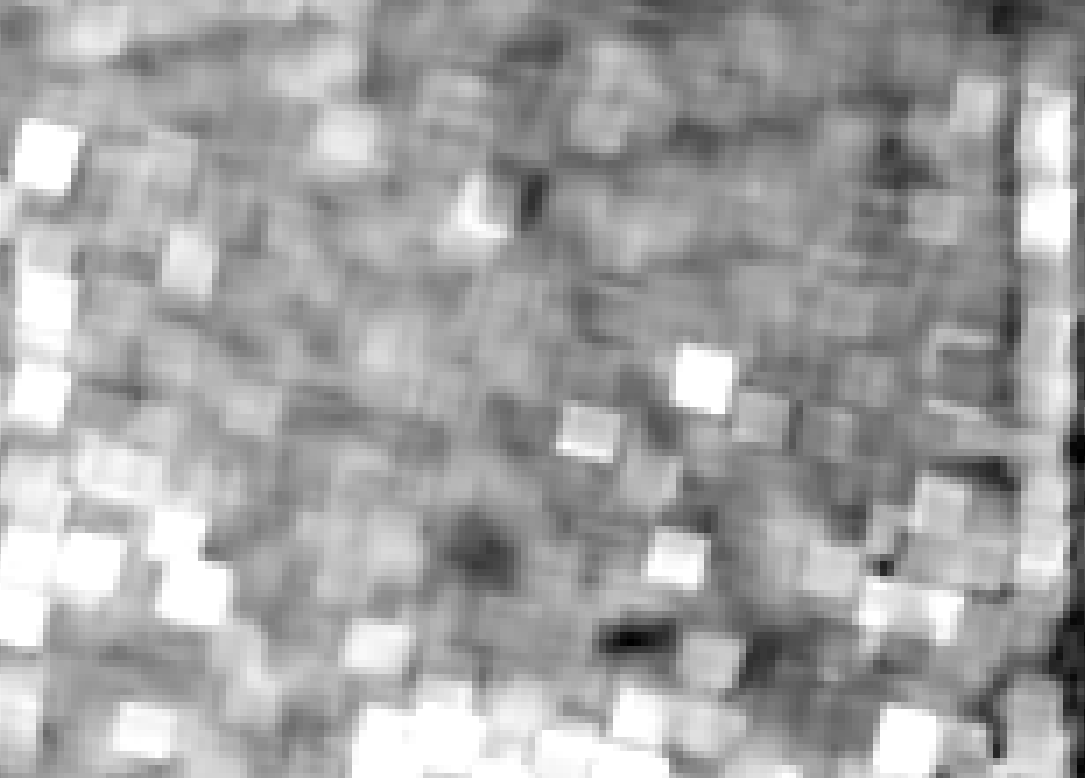
\includegraphics[width=.33\textwidth]{images/resolution_examples/coh_post.png}};}

\node[below=of a]{\small very high resolution};
\node[below=of b]{\small optical};
\node[below=of c]{\small radar};

\end{tikzpicture}

\end{frame}


\begin{frame}
\frametitle{Multi$^3$Net}

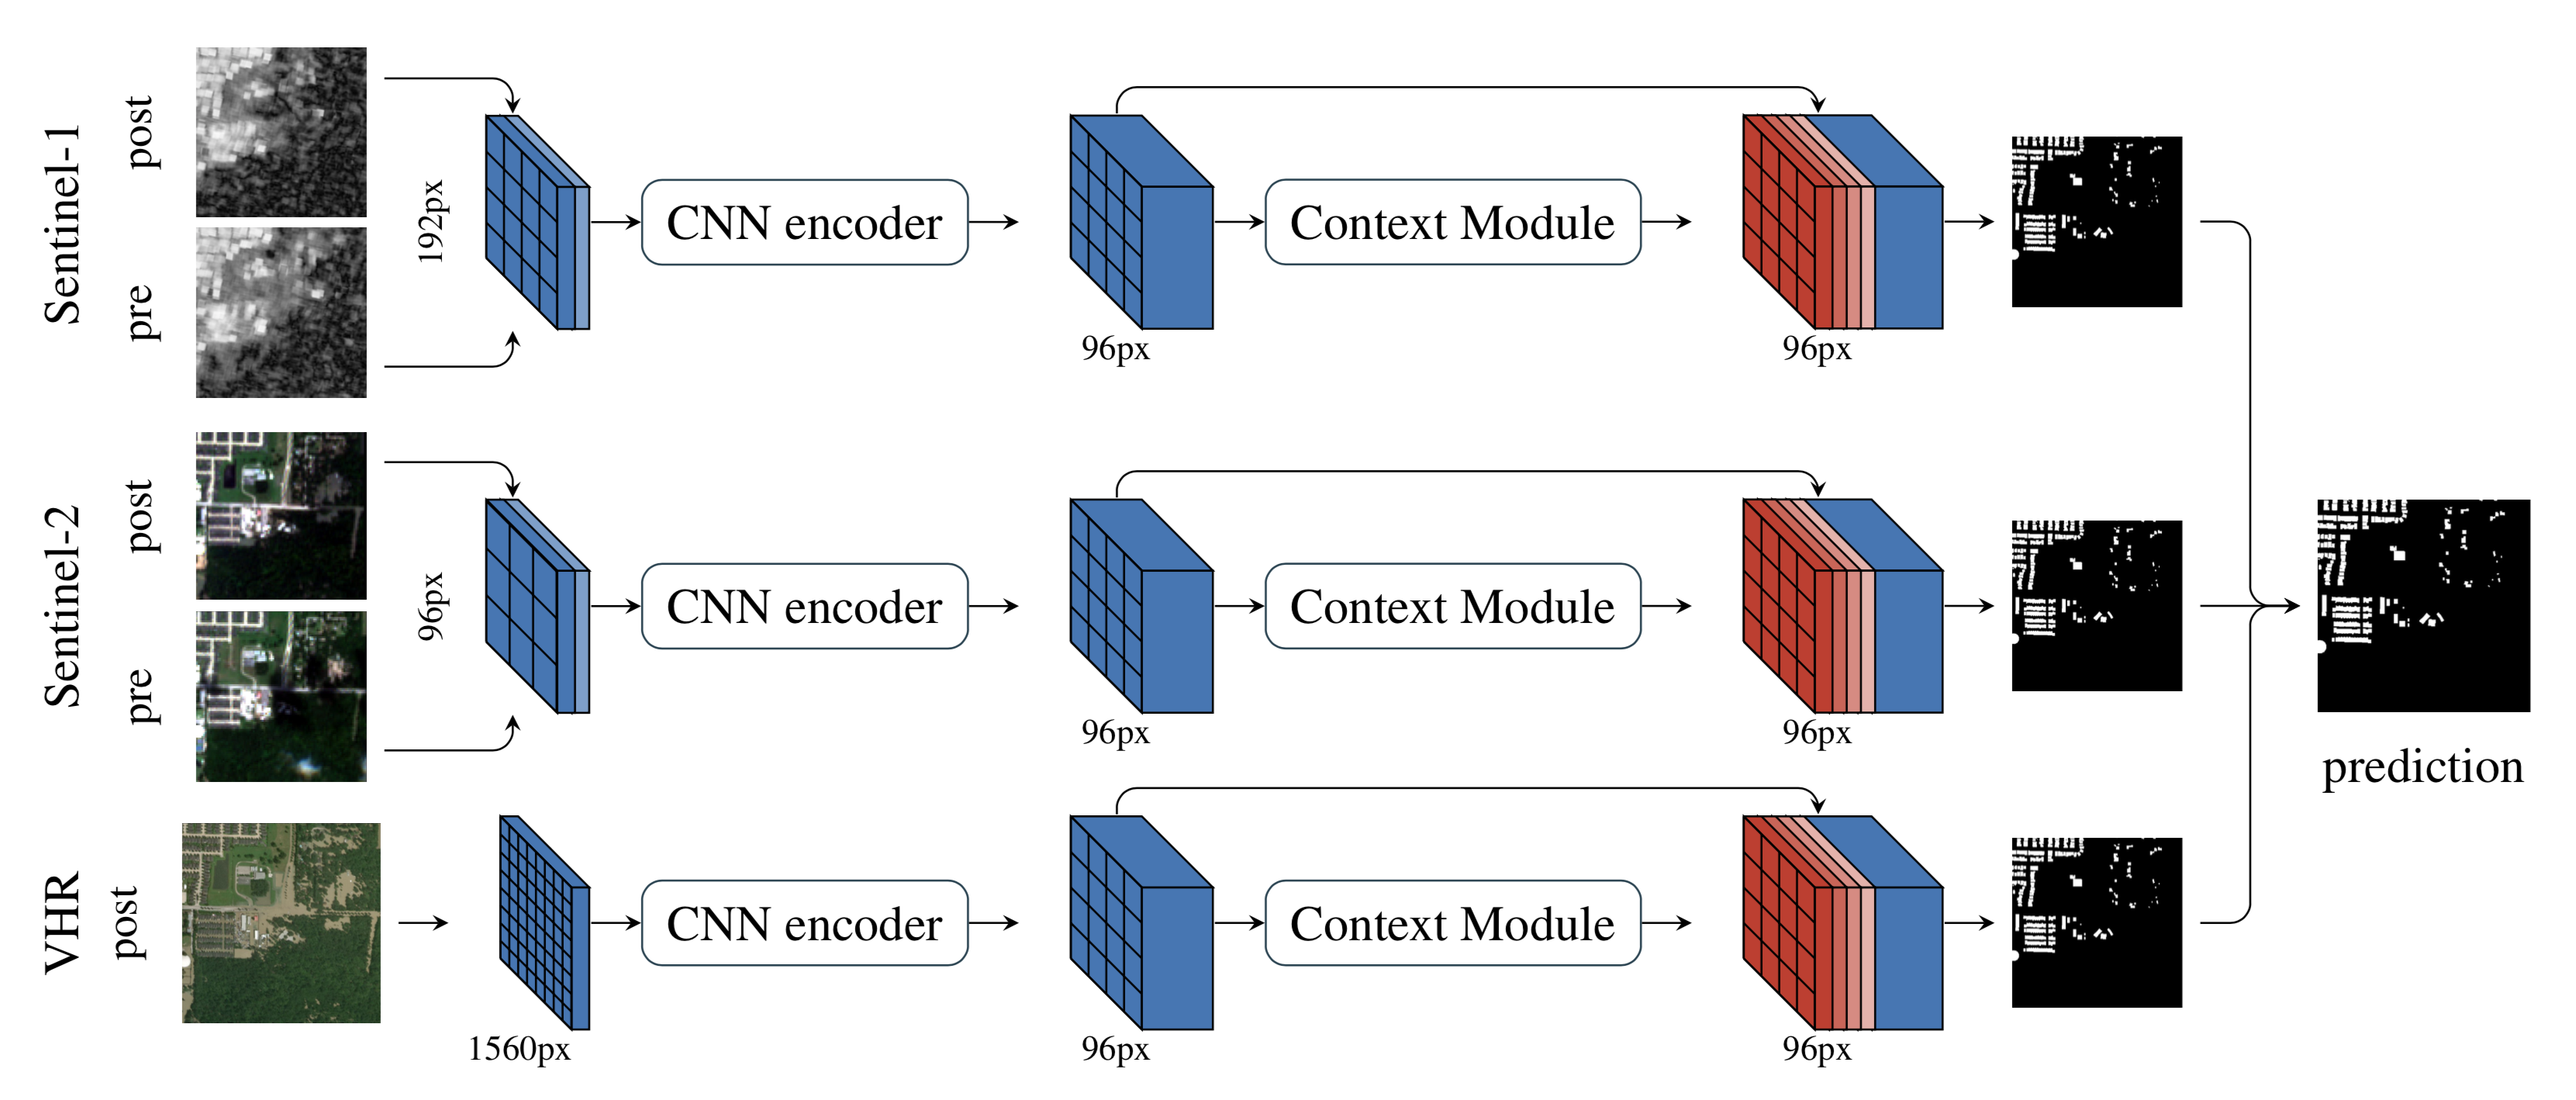
\includegraphics[width=\textwidth]{images/multi3net}


%



\tikzstyle{perspective3d}=[z={(0.5cm,-0.5cm)}, x={(1cm,0cm)}, y={(0cm,1cm)}]
\tikzstyle{conn}=[-stealth, rounded corners]
\tikzstyle{shared}=[stealth-stealth, rounded corners, very thick]
\tikzstyle{fm}=[inner sep=0]
\tikzstyle{h}=[]
\tikzstyle{net}=[inner sep=.5em, draw=gridcolor, rounded corners]
\tikzstyle{grid}=[inner sep=0]

\newcommand{\mygrid}[2]{%
        \begin{tikzpicture}[perspective3d, scale=.8*#2]
            \begin{scope}[canvas is yz plane at x=0]
            \draw[fill=activationcolor] (0,0) rectangle (1,1);
            \draw[step=#1, draw=black] (0,0)  grid (1,1);
            \end{scope}
        \end{tikzpicture}    
        }%

\newcommand{\mygridd}[3]{%
        \def\scale{#1}
        \def\depth{#2}
        \def\step{#3}

        \begin{tikzpicture}[perspective3d, scale=\scale]
            
            \draw[canvas is xy plane at z=1, fill=activationcolor] (0,0) -- (0,1) -- (\depth,1) -- (\depth,0) -- (0,0);
            \draw[canvas is xz plane at y=1, fill=activationcolor] (0,0) -- (0,1) -- (\depth,1) -- (\depth,0) -- (0,0);
            \draw[canvas is yz plane at x=0, fill=activationcolor] (0,0) -- (0,1) -- (1,1) -- (1,0) -- (0,0);
            \draw[canvas is yz plane at x=0, step=\step, draw=black] (0,0)  grid (1,1);
            
        \end{tikzpicture}    
        }%

\newcommand{\splitgrid}{%
        \def\scale{1}
        \def\depth{.5}
        \def\step{.1}

        \begin{tikzpicture}[perspective3d, scale=\scale]
            
            \draw[canvas is xy plane at z=1, fill=activationcolor] (0,0) -- (0,1) -- (\depth,1) -- (\depth,0) -- (0,0);
            \draw[canvas is xz plane at y=1, fill=activationcolor] (0,0) -- (0,1) -- (\depth,1) -- (\depth,0) -- (0,0);
            \draw[canvas is yz plane at x=0, fill=activationcolor] (0,0) -- (0,1) -- (1,1) -- (1,0) -- (0,0);
            \draw[canvas is yz plane at x=0, step=\step, draw=black] (0,0)  grid (1,1);
            
        \end{tikzpicture}    
        }

\newcommand{\mygridfour}[3]{%
        \def\scale{#1}
        \def\depth{#2}
        \def\step{#3}

        \begin{tikzpicture}
            
            \node{\mygridd{\scale}{\depth}{\steps}};            

        \end{tikzpicture}    
        }%

\newcommand{\myimage}[2]{%
        \begin{tikzpicture}
            %\begin{scope}[canvas is yz plane at x=0]
                \node[]{\includegraphics[#1]{#2}};
            %\end{scope}
        \end{tikzpicture}    
        }%

\newcommand{\vhrdownnet}{
\begin{tikzpicture}[node distance=1em]
\node[fm, label={above:\tiny0.625m}](vhr1){\mygrid{0.03125}{2}};
\node[right=of vhr1, fm, label={above:\tiny1.25m}](vhr2){\mygrid{0.0625}{2}};
\node[right=of vhr2, fm, label={above:\tiny2.5m}](vhr3){\mygrid{0.125}{2}};
\node[right=of vhr3, fm, label={above:\tiny5m}](vhr4){\mygrid{0.25}{2}};
\node[right=of vhr4, fm, label={above:\tiny10m}](vhr5){\mygrid{0.5}{2}};

\draw[conn] (vhr1.center) -- (vhr2);
\draw[conn] (vhr2.center) -- (vhr3);
\draw[conn] (vhr3.center) -- (vhr4);
\draw[conn] (vhr4.center) -- (vhr5);
\end{tikzpicture}
}

\newcommand{\classnet}{
\begin{tikzpicture}[node distance=0.5em]

\node(d1)[fm]{\mygrid{0.1}{2}};
\node(d2)[fm, right=of d1]{\mygrid{0.125}{1.8}};
\node(d3)[fm, right=of d2]{\mygrid{0.25}{1.6}};
\node(d4)[fm, right=of d3]{\mygrid{0.3333}{1.3}};
\node(c)[fm, right=of d4]{\mygrid{0.5}{1}};
\node(u4)[fm, right=of c]{\mygrid{0.3333}{1.3}};
\node(u3)[fm, right=of u4]{\mygrid{0.25}{1.6}};
\node(u2)[fm, right=of u3]{\mygrid{0.125}{1.8}};
\node(u1)[fm, right=of u2]{\mygrid{0.1}{2}};

\draw[conn] (d1.center) -- (d2);
\draw[conn] (d2.center) -- (d3);
\draw[conn] (d3.center) -- (d4);
\draw[conn] (d4.center) -- (c);
\draw[conn] (c.center) -- (u4);
\draw[conn] (u4.center) -- (u3);
\draw[conn] (u3.center) -- (u2);
\draw[conn] (u2.center) -- (u1);

\draw[conn] (d1.north) |- ++(1,.5) -| (u1.north);
\draw[conn] (d2.north) |- ++(1,.5) -| (u2.north);
\draw[conn] (d3.north) |- ++(1,.5) -| (u3.north);
\draw[conn] (d4.north) |- ++(1,.5) -| (u4.north);


\end{tikzpicture}
}

\newcommand{\stwoupnet}{
\begin{tikzpicture}[node distance=1em
\node[fm, label={left:$\text{S2}_{10m}$}](s210){\mygrid{0.125}{1}};
\node[above=of s210, fm, label={left:$\text{S2}_{20m}$}](s220){\mygrid{0.25}{1}};
\node[above=of s220, fm, label={left:$\text{S2}_{60m}$}](s260){\mygrid{.5}{1}};

\node[right=of s260, fm](s260_60_1){\mygrid{.25}{1}};
\node[right=of s260_60_1, fm](s260_60_2){\mygrid{.125}{1}};

\node[right=of s220, fm](s220_20_1){\mygrid{.125}{1}};

\node[right=6em of s220, fm](y){\mygrid{.125}{1}};

\draw[conn] (s210) -| (y);
\draw[conn] (s220) -- (s220_20_1) -- (y);
\draw[conn] (s260) -- (s260_60_1) -- (s260_60_2) -| (y);

\end{tikzpicture}

}

\newcommand{\stwoupsample}{

\begin{tikzpicture}

\node[fm, label={left:$\text{S2}_{10m}$}](s210){\mygrid{0.125}{1}};
\node[above=of s210, fm, label={left:$\text{S2}_{20m}$}](s220){\mygrid{0.25}{1}};
\node[above=of s220, fm, label={left:$\text{S2}_{60m}$}](s260){\mygrid{.5}{1}};

\coordinate[right=of s210] (preout);

\node[right=.2em of preout, fm](out10){\mygrid{0.125}{1}};
\node[right=.2em of out10, fm](out20){\mygrid{0.125}{1}};
\node[right=.2em of out20, fm](out60){\mygrid{0.125}{1}};

\draw[conn] (s210) -- (out10);
\draw[conn] (s220) -| (out20);
\draw[conn] (s260) -| (out60);

\end{tikzpicture}

}

\newcommand{\concat}{
    \begin{tikzpicture}
    \node[h](a) at (0,0){\mygrid{0.125}{1}};
    \node[h](b) at (-0.1,0){\mygrid{0.125}{1}};
    \node[h](c) at (-0.2,0){\mygrid{0.125}{1}};
    \end{tikzpicture}
}

\tikzset{pic shift/.store in=\shiftcoord,
	pic shift={(0,0)},
	pics/vhrbaseline_detailed/.style={
		code={

            \node[label={[align=center]below: \small Input}] (input) {\includegraphics[width=1.5cm]{\vhrimage}};
            
            \node[net,right=of input, align=center] (resnet) {CNN \\ (ResNet)};
            \only<1>{
            \node[h, right=of resnet, inner sep=0, label={[align=center]below: \small classifier}] (h0) {
                %\mygrid{0.25}{1}
                %\mygridd{1}{.5}{.25}
                \includegraphics[width=2cm]{images/histogram.png}
                };
            }
            \draw[conn] (input.east) -- (resnet);
            \draw[conn] (resnet) -- (h0);
            
                        
            \visible<2->{
            \node[h, right=of resnet, inner sep=0, label={[align=center]below: \small Feature \\ \small Maps}] (h0) {
                \mygridd{1}{.5}{.25}
                };
            }

            \visible<3->{
            \node[right=of h0] (pspnet) {\resizebox{!}{5cm}{\figpspmodule}};
            \node[h, right=.5em of pspnet, inner sep=0, label={[align=center]below: \small Feature\\ \small Maps}] (h3) {\mygridd{1}{1}{.25}};
            }

            \visible<2>{
            \node[h, right=of h3, label={[align=center]below: \small Output}] (out) {\includegraphics[width=1.5cm]{\labelimage}};
            \node[net, align=center] (pspnetabstract) at ($ (h0)!0.5!(out) $){PSP\\Decoder};
            \phantom{\node[right=of h0] (pspnet) {\resizebox{!}{5cm}{\figpspmodule}};}
            \phantom{\node[h, right=.5em of pspnet, inner sep=0, label={[align=center]below: \small Feature\\ \small Maps}] (h3) {\mygridd{1}{1}{.25}};}
            \draw[conn] (h0) -- (pspnetabstract);
            \draw[conn] (pspnetabstract) -- (out);
            
            }

            \visible<3->{
            \draw[conn] (h0) -- (pspnet);
            \draw[conn] (pspnet) -- (h3);
            \node[h, right=of h3, label={[align=center]below: \small Output}] (out) {\includegraphics[width=1.5cm]{\labelimage}};
            \draw[conn] (h3) -- (out);
            \draw[conn] (h0) |- ++(2em, 7em) -| (h3);
            }

		}
	}
}


\tikzset{pic shift/.store in=\shiftcoord,
	pic shift={(0,0)},
	pics/vhrbaseline/.style={
		code={

            % \includegraphics[width=1.2cm]{\vhrimage} 
            \node[] (input) {\includegraphics[width=1.2cm]{\vhrimage}};
            \node[net,right=3.8em of input] (resnet) {ResNet};
            \node[h, right=of resnet] (h0) {\mygrid{0.25}{1}};
            \node[net,right=of h0, align=left] (pspnet) {PSP\\Module};
            \node[h,right=of pspnet, align=left] (pspout) {\includegraphics[width=1.2cm]{\labelimage}};
            %\node[h, right=of pspout] (h3) {\concat};
            
            %\node[h, right=of h3] (out) {\includegraphics[width=1.3cm]{\labelimage}};
            
            %\draw[conn] (resnet.north) |- ++(1,1) -| (h1.north);
            %\draw[conn] (resnet.north)++(-.1,0) |- ++(1,1.1)  node [near end, above, xshift=3em]{\tiny skip} -| (h3.north);
            %\draw[conn] (resnet.north)++(-.2,0) |- ++(1,1.2) -| (h3.north);
            
            \draw[conn] (input.east) -- (resnet);
            \draw[conn] (resnet) -- (h0);
            \draw[conn] (h0) -- (pspnet);
            \draw[conn] (pspnet) -- (pspout);
            %\draw[conn] (pspout) -- (h3);
            %\draw[conn] (h3) -- (out);

		}
	}
}

\tikzset{pic shift/.store in=\shiftcoord,
	pic shift={(0,0)},
	pics/inputstreammono/.style={
		code={

            % \includegraphics[width=1.2cm]{\vhrimage} 
            \node[net] (resnet) {ResNet};
            \node[h, right=of resnet] (h0) {\mygrid{0.25}{1}};
            \node[net, right=of h0, align=left] (pspnet) {
                PSP \\ Module
            };
            \node[h, right= of pspnet, label={below:\tiny 96px}] (h3) {\concat};
            
            %\node[h, right=of h3] (out){\includegraphics[width=1.3cm]{\labelimage}};
            
            %\draw[conn] (resnet.north) |- ++(1,1) -| (h1.north);
            %\draw[conn] (resnet.north)++(-.1,0) |- ++(1,1.1)  node [near end, above, xshift=3em]{\tiny skip} -| (h3.north);
            %\draw[conn] (resnet.north)++(-.2,0) |- ++(1,1.2) -| (h3.north);
            
            %\draw[conn] (input.east) -- (resnet);
            \draw[conn] (resnet) -- (h0);
            \draw[conn] (h0) -- (pspnet);
            \draw[conn] (pspnet) -- (h3);
            %\draw[conn] (h3) -- (out);

		}
	}
}

\tikzset{pic shift/.store in=\shiftcoord,
	pic shift={(0,0)},
	pics/unet/.style={
		code={
            \def\s{0.5}

            \node(d1)[fm]{\mygrid{0.1*\s}{2*\s}};
            \node(d2)[fm, right=of d1]{\mygrid{0.125*\s}{1.8*\s}};
            \node(d3)[fm, right=of d2]{\mygrid{0.25*\s}{1.6*\s}};
            %\node(d4)[fm, right=of d3]{\mygrid{0.3333*\s}{1.3*\s}};
            \node(c)[fm, right=of d3]{\mygrid{0.5*\s}{1*\s}};
            %\node(u4)[fm, right=of c]{\mygrid{0.3333*\s}{1.3*\s}};
            \node(u3)[fm, right=of c]{\mygrid{0.25*\s}{1.6*\s}};
            \node(u2)[fm, right=of u3]{\mygrid{0.125*\s}{1.8*\s}};
            \node(u1)[fm, right=of u2]{\mygrid{0.1*\s}{2*\s}};
            
            \draw[conn] (d1.center) -- (d2);
            \draw[conn] (d2.center) -- (d3);
            \draw[conn] (d3.center) -- (c);
            %\draw[conn] (d4.center) -- (c);
            \draw[conn] (c.center) -- (u3);
            %\draw[conn] (u4.center) -- (u3);
            \draw[conn] (u3.center) -- (u2);
            \draw[conn] (u2.center) -- (u1);
            
            \draw[conn] (d1.north) |- ++(1*\s,.5*\s) -| (u1.north);
            \draw[conn] (d2.north) |- ++(1*\s,.5*\s) -| (u2.north);
            \draw[conn] (d3.north) |- ++(1*\s,.5*\s) -| (u3.north);
            %\draw[conn] (d4.north) |- ++(1*\s,.5*\s) -| (u4.north);
		}
	}
}



\tikzset{pic shift/.store in=\shiftcoord,
	pic shift={(0,0)},
	pics/s2damagenet/.style={
		code={

            \coordinate (center) at (0,0);
            
            % \includegraphics[width=2cm]{\vhrimage} 
            \node[above=-.6em of center, label={[label distance=0em, rotate=0]left:\small pre}] (inputpre) {\myimage{width=1.2cm}{\preimage}};
            
            \node[below=-.6em of center, label={[label distance=0em, rotate=0]left:\small post}] (inputpost) {\myimage{width=1.2cm}{\postimage}};
            
            \node[right=3em of center] (minus) {
            \begin{tikzpicture}
                \node[inner sep=0] at (0,0){\mygrid{0.25}{1}};
                \node[inner sep=0] at (-.1,0){\mygrid{0.25}{1}};
            \end{tikzpicture}
            };

            \node[net,right=of minus] (resnet) {ResNet};
            \node[right=of resnet] (h0) {\mygrid{0.25}{1}};
            
            \node[net, right=of h0, align=left] (h1) {PSP\\Module};
            \node[h, right=of h1] (h2) {
                %\mygrid{0.125}{1}
                \includegraphics[width=1.2cm]{\labelimage}
            };
            
            %\draw[shared]  (resnetpost) -- (resnetpre) node[midway, left]{\tiny $\textbf{W}$};

            \draw[conn] (inputpre.east)++(0,1em) -| (minus);
            \draw[conn] (inputpost.east)++(0,-1em) -| (minus);
            \draw[conn] (minus) -- (resnet);
            \draw[conn] (resnet) -- (h0);
            \draw[conn] (h0) -- (h1);
            \draw[conn] (h1) -- (h2);

		}
	}
}



\tikzset{pic shift/.store in=\shiftcoord,
	pic shift={(0,0)},
	pics/s2damagenetold/.style={
		code={

            \coordinate (center) at (0,0);
            
            % \includegraphics[width=2cm]{\vhrimage} 
            \node[above=-.4em of center, label={[label distance=0em, rotate=0]left:\small pre}] (inputpre) {\myimage{width=1.2cm}{\preimage}};
            \node[net,right=of inputpre] (resnetpre) {ResNet};
            \node[right=of resnetpre] (h0pre) {\mygrid{0.25}{1}};
            
            \node[below=-.4em of center, label={[label distance=0em, rotate=0]left:\small post}] (inputpost) {\myimage{width=1.2cm}{\postimage}};
            \node[net,right=of inputpost] (resnetpost) {ResNet};
            \node[right=of resnetpost] (h0post) {\mygrid{0.25}{1}};
            
            \coordinate (centerend) at ($ (h0pre.east)!0.5!(h0post.east) $);
            
            \node[right=of centerend] (minus) {
            \begin{tikzpicture}
                \node[inner sep=0] at (0,0){\mygrid{0.25}{1}};
                \node[inner sep=0] at (.1,0){\mygrid{0.25}{1}};
            \end{tikzpicture}
            };
            
            \node[h, right=of minus] (h1) {\mygrid{0.125}{1}};
            \node[h, right=of h1] (h2) {\mygrid{0.125}{1}};
            
            \draw[shared]  (resnetpost) -- (resnetpre) node[midway, left]{\tiny $\textbf{W}$};

            \draw[conn] (inputpre) -- (resnetpre);
            \draw[conn] (resnetpre) -- (h0pre);
            \draw[conn] (h0pre) -| (minus);
            \draw[conn] (inputpost) -- (resnetpost);
            \draw[conn] (resnetpost) -- (h0post);
            \draw[conn] (h0post) -| (minus);
            
            \draw[conn] (minus) -- (h1);
            \draw[conn] (h1) -- (h2);

		}
	}
}

\newcommand{\figpspmodule}{
    \begin{tikzpicture}[node distance=.5em]
    
    \begin{scope}[xscale=1.5, yscale=-1.25]
    
    \node(pool) at (-1.2,2.1) {pool};
    %\node(upsample) at (3.5,1.5) {upsample};
    
    \node[grid](grid1) at (0,0){\mygridd{.3}{.5}{.5}};
    \node[grid](grid2) at (0,.8){\mygridd{.5}{.5}{.25}};
    \node[grid](grid3) at (0,1.8){\mygridd{.75}{.5}{.25}};
    \node[grid](grid16) at (0,3){\mygridd{1}{.5}{.25}};
    
    \coordinate[below right= 1em and 2em of grid16](convcoord);
    
    \node(conv1) at (1,0) {conv};
    \node(conv2) at (1,.8) {conv};
    \node(conv3) at (1,1.8) {conv};
    \node(conv16) at (1,3) {conv};
    
    \node[grid](gridd1) at (2,0){\mygridd{.3}{.2}{.5}};
    \node[grid](gridd2) at (2,.8){\mygridd{.5}{.2}{.25}};
    \node[grid](gridd3) at (2,1.8){\mygridd{.75}{.2}{.25}};
    \node[grid](gridd16) at (2,3){\mygridd{1}{.2}{.25}};
    
    \end{scope}
    
    \draw[conn] (pool) -- ++(2em,0) |- (grid1);
    \draw[conn] (pool) -- ++(2em,0) |- (grid2);
    \draw[conn] (pool) -- ++(2em,0) |- (grid3);
    \draw[conn] (pool) -- ++(2em,0) |- (grid16);
    
    \draw[conn] (grid1) -- (conv1) -- (gridd1);
    \draw[conn] (grid2) -- (conv2) -- (gridd2);
    \draw[conn] (grid3) -- (conv3) -- (gridd3);
    \draw[conn] (grid16) -- (conv16) -- (gridd16);
    
    %\draw[conn] (gridd1) -- ++(2em,0) |- (upsample);
    %\draw[conn] (gridd2) -- ++(2em,0) |- (upsample);
    %\draw[conn] (gridd3) -- ++(2em,0) |- (upsample);
    %\draw[conn] (gridd16) -- ++(2em,0) |- (upsample);
    
    \node[draw, rounded corners, label={[align=center]below:Pyramid Spatial Pooling (PSP) \\ Module}, fit=(pool)(grid1)(gridd16)]{};
    
    %\node[right=of upsample]{\mygridfour{1}{.2}{.25}};
    
    \end{tikzpicture}
}
%
%\begin{tikzpicture}[node distance=.75em, scale=1]
%
%\def\vhrimage{images/tile/vhr}
%\def\labelimage{images/tile/flooded}
%\def\labelimage{images/tile/buildings}
%\draw pic (base) at (0,0) {vhrbaseline};
%
%\def\preimage{images/tile/coh_int_20170706_20170823}
%\def\postimage{images/tile/coh_int_20170823_20170904}
%\draw pic (s2damagenet) at (0,2.1) {s2damagenet};
%%\coordinate (c1) at ($ (s2damageneth2)!0.5!(baseh3) $);
%%\draw[conn] (s2damageneth2) -| ($ (baseh3.north) + (-.2em,0) $);
%
%\def\preimage{images/tile/s2pre}
%\def\postimage{images/tile/s2post}
%\draw pic (s2damagenetsar) at (0,4.7) {s2damagenet};
%%\draw[conn] (s2damagenetsarh2) -| ($ (baseh3.north) + (.2em,0) $);
%
%\node[right=3em of s2damageneth2](out){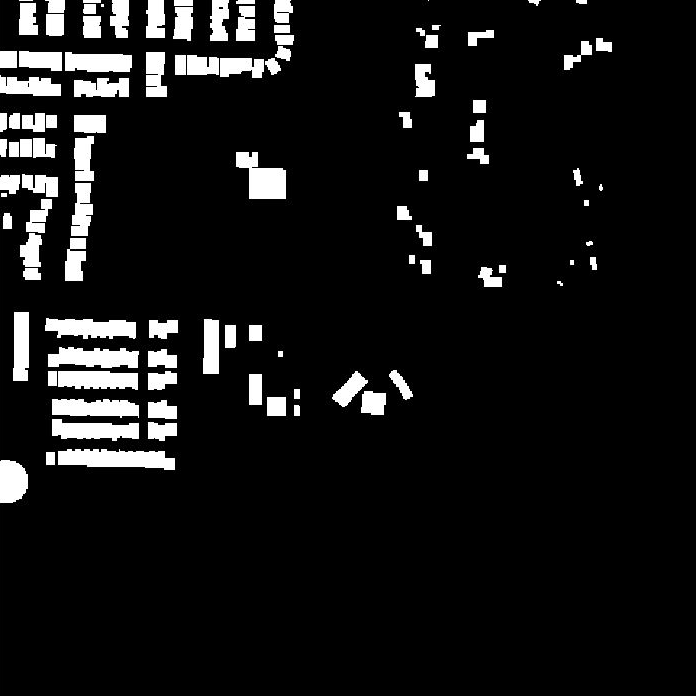
\includegraphics[width=1.2cm]{images/tile/buildings}};
%
%\draw[conn] (s2damageneth2) -- (out);
%\draw[conn] (s2damagenetsarh2) -| ($ (s2damagenetsarh2.east)!0.5!(out.west) $) |- (out.west);
%\draw[conn] (basepspout) -| ($ (basepspout.east)!0.5!(out.west) $) |- (out.west);
%
%\end{tikzpicture}


\end{frame}

\begin{frame}
\frametitle{Publications and Code}



\textbf{AAAI 2019 Conference Paper:}

{\small
Rudner, T. G., Rußwurm, M., Fil, J., Pelich, R., Bischke, B., Kopackova, V., \& Bilinski, P. (2019). Multi $^{\mathbf {3}} $ Net: Segmenting Flooded Buildings via Fusion of Multiresolution, Multisensor, and Multitemporal Satellite Imagery. Association for the Advancement of Artificial Intelligence AAAI-19.}

\vspace{2em}

\textbf{2 NeurIPS Workshop Papers} at \textbf{AI for Social Good} and \textbf{Spatio-Temporal Workshops}.

%\vspace{1em}
%
%\textbf{NeurIPS18 Spatio-Temporal Workshop:}\\
%{\small
%Fil, J., Rudner, T. G., Russwurm, M., Bischke, B., Pelich, R., Kopackova, V., \& Bilinski, P. (2018). Multi³Net: Segmenting Flooded Buildings via Fusion of Multiresolution, Multisensor, and Multitemporal Satellite Imagery. NeurIPS18 Spatio-Temporal Workshop}
%
%\vspace{1em}
%
%\textbf{NeurIPS18 AI for Social Good Workshop:}\\
%{\small
%Rudner, T. G., Rußwurm, M., Fil, J., Pelich, R., Bischke, B., \& Kopacková, V. Rapid Computer Vision-Aided Disaster Response via Fusion of Multiresolution, Multisensor, and Multitemporal Satellite Imagery. NeurIPS18 AI for Social Good Workshop.
%}

\vspace{1em}
\textbf{GitHub}
\url{https://github.com/FrontierDevelopmentLab/multi3net}

\end{frame}